% or aspectratio=43
\documentclass[aspectratio=169]{beamer}

% remove this line for an english presentation
%\usepackage{ngerman}

% Optional arguments (separate by comma):
% darkmode			- Black background and white font
% imagetitlepage	- Adds the images defined in \titlegraphic to the title page
\usepackage[imagetitlepage]{lgdv/lgdv_beamer}

\usepackage{mdframed}

\usepackage{xcolor}
\graphicspath{{images/}}

%make existing function names bold
\lstset%
{%
	%
	% Custom Types for Syntax Highlighting
	%
	emph=[0]%
	{%
		Maxr
	},
	emphstyle=[0]{\bfseries\color{typecolor}},
}

\subtitle{AGPhys WS 20/21}
\title{Parallel Algorithms - Implementation and Usage}
\author[Darius Rückert]{Darius Rückert}
\date{\today}

\titlegraphic
{
	\begin{figure}[!h]
					
\includegraphics[height=.3\textheight]{cuda}
					\hfill
					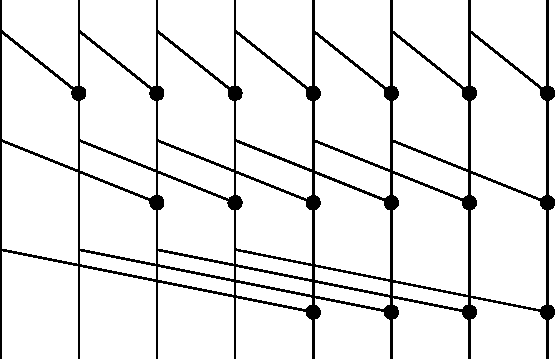
\includegraphics[height=.3\textheight]{warpscan}
					\hfill
					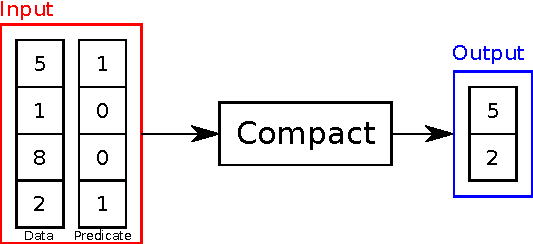
\includegraphics[height=.3\textheight]{o_compact}
	\end{figure}
}

\begin{document}

\frame
{
	\titlepage
}

\frame
{
\frametitle{Outline}
\begin{itemize}
	\item Reduce 
	\item Scan 
	\item Scatter
	\item Gather
	\item Compact
	\item Sort
\end{itemize}
}



\begin{frame}[fragile]
\frametitle{Reduce}
\begin{figure}
	\centering
	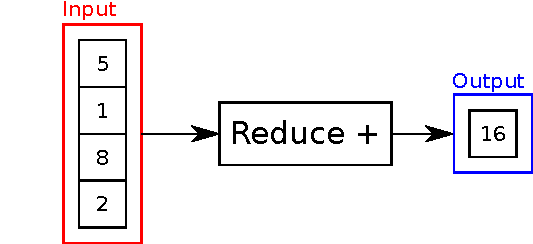
\includegraphics[height=0.6\textheight]{o_reduce}
\end{figure}

\begin{lstlisting}
// Sum over all elements in data
float sum = thrust::reduce(data.begin(),data.end());
\end{lstlisting}
\end{frame}



\begin{frame}[fragile]
	\frametitle{Reduce}
	Sequential implementation on the CPU:
\begin{lstlisting}
T reduce(vector<T> input, OP reduce_op, T initial_value = T())
{
	T output = initial_value;
	for(auto v : input)
	{
		output = reduce_op(output, v);
	}
	return output;
}
\end{lstlisting}
\end{frame}

\frame
{	
	\frametitle{Reduce}
	\begin{itemize}
		\item An input array is reduced to a single element of \textbf{the same type}
		\item<2-> A \textbf{commutative} reduce operation merges two elements to one
		\item<2-> Typical operations:
		\begin{itemize}
			\item add
			\item min/max
			\item multiply add (vector dot-product)
		\end{itemize}
	\end{itemize}
}


\frame
{	
	\frametitle{Reduce CUDA Implementation}
	\begin{itemize}
		\item Make use of the 3-level hierarchy:
		\begin{enumerate}
			\item Warp Reduce
			\item Block Reduce
			\item Global Reduce
		\end{enumerate}	
	\end{itemize}
\begin{figure}
	\centering
	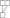
\includegraphics[height=0.3\textheight]{reduce}
\end{figure}
}


\frame
{	
	\frametitle{Warp Reduce}
	\begin{itemize}
		\item Each thread in a warp has one element
		\item The number of elements is halfed in each step
		\item After $\log_2(N)$ a single element remains
		\item Communication between threads with \texttt{shuffle} instructions
	\end{itemize}
}


\begin{frame}[fragile]
\frametitle{Warp Reduce}
\begin{figure}
	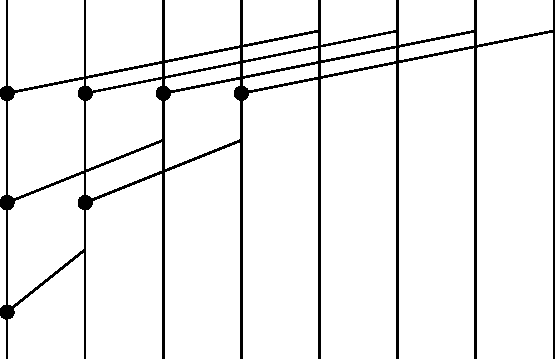
\includegraphics[height=0.5\textheight]{warpreduce}
\end{figure}
\begin{lstlisting}
val += __shfl_down_sync(0xFFFFFFFF, val, 4);
val += __shfl_down_sync(0xFFFFFFFF, val, 2);
val += __shfl_down_sync(0xFFFFFFFF, val, 1);
\end{lstlisting}

\end{frame}




\begin{frame}[fragile]
\frametitle{Warp Reduce}
\begin{itemize}
	\item Shuffle warp reduce with 32-threads
	\item Different reduce operators can be used in line 6
\end{itemize}

\begin{lstlisting}
T warpReduceSum(T val)
{
	for (unsigned int offset = warpSize >> 1; offset > 0; offset >>= 1)
	{
		auto v = __shfl_down_sync(0xFFFFFFFF, val, offset);
		val = val + v;
	}
	return val;
}
\end{lstlisting}

\end{frame}

\begin{frame}[fragile]
\frametitle{Block Reduce}
\begin{itemize}
	\item A block consists of multiple warps
	\item<2->[$\rightarrow$] Reduce to one element per block
	\item<3->[$\rightarrow$] Use shared memory for fast in-block communication
\end{itemize}


\end{frame}

\begin{frame}[fragile]
\frametitle{Block Reduce}
\begin{itemize}
	\item Implementation with atomic operations (part 1)
\end{itemize}

\begin{lstlisting}
// Final block sum
__shared__ T blockSum;

// The first thread in the block initializes the result
if(threadIdx.x == 0) blockSum = T(0);

// Make sure the shared memory is initialized for all warps
__syncthreads();

auto v = data[ti.thread_id];
v = blockReduceSum(v,blockSum);
\end{lstlisting}
\end{frame}


\begin{frame}[fragile]
\frametitle{Block Reduce}
\begin{lstlisting}
T blockReduceSum(T val, T& blockSum)
{
	// Shuffle reduce in registers (see previous slides)
	val = warpReduceSum(val);

	// The first thread in each warp contatins the local sum
	// -> Reduce in smem with atomic add
	if (threadIdx.x & (WARP_SIZE-1) == 0)
		atomicAdd(&blockSum,val);
		
	// Wait until all warps called atomicAdd
	__syncthreads();

	return blockSum;
}
\end{lstlisting}
\end{frame}

\begin{frame}[fragile]
\frametitle{Global Reduce}
\begin{itemize}
	\item A kernel launches multiple blocks
	\item<2-> Intra-block communication through global memory
	\item<3->[$\rightarrow$] Each blocks calls atomicAdd to the result in global memory
\end{itemize}


\end{frame}


\begin{frame}[fragile]
\frametitle{Global Reduce}
\begin{itemize}
	\item Implementation with atomics:
\end{itemize}

\begin{lstlisting}
__shared__ T blockSum;

// One element per thread
auto v = data[ti.thread_id];

// Reduce all values from this block
v = blockReduceSum(v,blockSum);

// The first thread in each block writes to global memory
if(ti.local_thread_id == 0)
	atomicAdd(output.data(),v);
\end{lstlisting}
\end{frame}


\frame
{	
	\frametitle{Non-Atomic Reduce Operations}
	\textbf{Problem}
	\begin{itemize}
		\item Not all reduce operations can be implemented with atomics!
		\item<2-> Some examples:
		\begin{itemize}
			\item Lexicographical Min/Max
			\item Key-value reduces
			\item[$\rightarrow$] Get the index of the particle with the highest momentum
		\end{itemize}		
	\end{itemize}
\onslide<3->
\textbf{Question}
	\begin{itemize}
	\item Is it still possible to globally reduce in a single kernel launch?
		\end{itemize}
}

\frame
{	
	\frametitle{Non-Atomic Warp Reduce}

\onslide<2->
	\begin{itemize}
		\item We can shuffle large structs with multiple 32-bit shuffle instructions
	\end{itemize}
\onslide<3->
	\textbf{Example}
	\begin{itemize}
	\item Shuffle both the key and data to other threads
	\item Reduce locally on the data
	\item[$\rightarrow$] Works for every type and all (custom) reduce operators
	
\end{itemize}	

}

\begin{frame}[fragile]
\frametitle{Non-Atomic Block Reduce}
Previous Implementation
\begin{itemize}
	\item Reduction with atomic operations to a single value in shared memory
		\item<2->[$\rightarrow$] Only works for atomic reduce operations (sum/min/max)
		\item<3->[$\rightarrow$] No custom operators or key-value reduces
\end{itemize}
\onslide<4->
Non-Atomic Implementation
\begin{itemize}
	\item<5-> Each warp writes the result to shared memory
	\item<6-> The first warp in the block reduces the intermediate results 
\end{itemize}



\end{frame}


\begin{frame}[fragile]
\frametitle{Non-Atomic Block Reduce}
\label{sl:nabr}

\begin{lstlisting}
// Each warp in a block needs one entry
__shared__ T shared[WARPS_PER_BLOCK];

// Warp reduce + write to smem
val = warpReduceSum(val);
if (lane == 0) shared[warpId] = val;
__syncthreads();

// The first warp loads the results from smem...
val = (threadIdx.x < BLOCK_SIZE / WARP_SIZE) ? shared[lane] : 0;
// ... and reduces the elements with shuffles
if (warpId==0) val = warpReduceSum(val); 
\end{lstlisting}
\end{frame}


\begin{frame}[fragile]
\frametitle{Non-Atomic Global Reduce}
\begin{itemize}
	\item Global synchronization is more complicated!
	\item<2-> We could either
	\begin{itemize}
		\item Block reduce, write to gmem, and launch a second kernel
		\item Build a global lock with atomics
	\end{itemize}
	\item<3->[$\rightarrow$] Global locks are very fast without conflicts
	\item<4->[$\rightarrow$] Only few conflicts occur, because only 1 thread per block acquires it
\end{itemize}

\end{frame}


\begin{frame}[fragile]
\frametitle{Non-Atomic Global Reduce}
\label{si:spinlock}
\begin{itemize}
	\item Reduction with atomic spin lock
\end{itemize}
\begin{lstlisting}
// After the block reduce...
if(threadIdx.x == 0)
{
	// Spin until lock==0 and set lock=1 (lock is an integer in gmem)
	while(atomicCAS(&lock,0,1) != 0) {}
	
	// Load from global memory, reduce, and write back
	T gv = output[0];
	v = reduce(v,gv); // reduce() can be a custom operator
	output[0] = v;
	
	// Release lock
	lock = 0;
}
\end{lstlisting}
\end{frame}

\begin{frame}[fragile]
\frametitle{Non-Atomic Global Reduce}
\label{si:spinlock}
\begin{itemize}
	\item Reduction with atomic spin lock
\end{itemize}
\begin{lstlisting}
// After the block reduce...
if(threadIdx.x == 0)
{
	// Spin until lock==0 and set lock=1 (lock is an integer in gmem)
	while(atomicCAS(&lock,0,1) != 0) {}
	
	// Load from global memory, reduce, and write back
	T gv = output[0];
	v = reduce(v,gv); // reduce() can be a custom operator
	output[0] = v;
	
	// Release lock
	lock = 0;
}
\end{lstlisting}
\end{frame}


\begin{frame}[fragile]
\frametitle{Thrust Reduce}
\begin{itemize}
	\item Thrust includes efficient global reduce implementations with
	\begin{itemize}
		\item custom reduce operators
		\item indirect reductions (reduce by key)
	\end{itemize}
	\item General reduce:
\end{itemize}
\begin{lstlisting}
thrust::device_vector<float> d_data;
float sum = thrust::reduce(d_data.begin(),d_data.end());
\end{lstlisting}
\begin{itemize}
	\item \href{https://thrust.github.io/doc/group__reductions.html}{Thrust Reduce API}
	
\end{itemize}
\end{frame}


\begin{frame}[fragile]
\frametitle{Thrust Reduce Variants}

\begin{itemize}
\begin{lstlisting}
thrust::reduce_by_key(keys_first, keys_last, values_first, 
		keys_output, values_output);		
\end{lstlisting}
	\item \texttt{reduce\_by\_key} is a generalization of reduce to key-value pairs.
\begin{lstlisting}
thrust::min_element(first, last);		
\end{lstlisting}	
	\item min\_element finds the smallest element in the range [first, last)
\begin{lstlisting}
thrust::max_element(first, last);		
\end{lstlisting}	
	\item max\_element finds the largest element in the range [first, last)
\end{itemize}
\end{frame}

\begin{frame}[fragile]
\frametitle{Thrust Reduce - Custom Operators}

\begin{lstlisting}
struct Particle{
	vec3 position;
	float radius = 0;
};

struct Maxr
{
	HD Particle operator()(const Particle& p1, const Particle& p2)
	{
		return p1.radius < p2.radius ? p2 : p1;
	}
};

\end{lstlisting}

\begin{lstlisting}
Particle p = thrust::reduce(ps.begin(),ps.end(),Particle(),Maxr());
cout << "Max radius = " << p.radius << endl;
\end{lstlisting}
\end{frame}


\begin{frame}[fragile]
\frametitle{Scan}
\begin{figure}
	\centering
	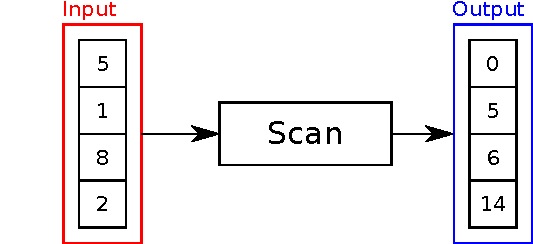
\includegraphics[height=0.6\textheight]{o_scan}
\end{figure}
\begin{lstlisting}
// Exclusive prefix sum
thrust::exclusive_scan(data.begin(),data.end(),output.begin());
\end{lstlisting}
\end{frame}


\begin{frame}[fragile]
	\frametitle{Scan}
	Sequential implementation on the CPU:
\begin{lstlisting}
void exclusive_scan(vector<T> input, vector<T>& output)
{
	T sum = 0;
	for(int i = 0; i < input.size(); ++i)
	{
		// Swap these two lines for an inclusive scan
		output[i] = sum;
		sum += input[i];
	}
}
\end{lstlisting}
\end{frame}

\begin{frame}[fragile]
	\frametitle{Scan}
	\begin{itemize}
		\item Each element in the output is the \textbf{sum of all previous elements} in the input
		\item<2-> Sequential implementation (exclusive scan):
\begin{lstlisting}
output[0] = T(0);
for(int i = 1; i < N; ++i)
{
	output[i] = output[i - 1] + input[i - 1];
}
\end{lstlisting}
\item<3-> \textbf{Problem:}
\begin{itemize}
	\item Each element depends on the previous element (line 4)
	\item[$\rightarrow$] Parallel implementation more difficult 
\end{itemize}

\end{itemize}
\end{frame}


\begin{frame}[fragile]
\frametitle{Scan}
Two different variants
\begin{itemize}
	\item \textbf{Inclusive Scan}: Sum of all previous elements \textbf{including} the current element
	\item \textbf{Exclusive Scan}: Sum of all previous elements \textbf{excluding} the current element
\end{itemize}
\onslide<2->
Implementation
\begin{enumerate}
	\item Compute inclusive scan for each warp
	\item Compute inclusive scan for each block
	\item Read last element from the previous block and add it
	\item[(4.)] Subtract input element if exclusive scan is required
\end{enumerate}
\end{frame}

\begin{frame}[fragile]
\frametitle{Warp Scan}
\begin{figure}
	\centering
	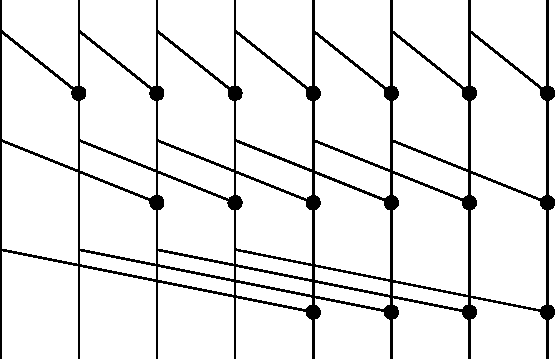
\includegraphics[height=0.6\textheight]{warpscan}
\end{figure}
\begin{lstlisting}
val += __shfl_up(val, 1);
val += __shfl_up(val, 2);
val += __shfl_up(val, 4);
\end{lstlisting}
\end{frame}


\begin{frame}[fragile]
\frametitle{Warp Scan}
\begin{itemize}
	\item Same as warp reduce, but in different direction and order
\end{itemize}

\begin{lstlisting}
T warpInclusiveScan(T val, unsigned int lane) 
{
	for (int d = 1; d < 32; d *= 2) 
	{
		T tmp = shfl_up(val,d);
		if (lane >= d) val += tmp;
	}
	return val;
}
\end{lstlisting}

\end{frame}


\begin{frame}[fragile]
\frametitle{Block Scan}
\begin{itemize}
	\item Similar to block reduce without atomics (see Slide \ref{sl:nabr})
\end{itemize}
\onslide<2->
\begin{enumerate}
	\item Warp scan + write to smem
	\item Warp scan in first warp + write to smem
	\item Each thread adds the scannend sum of the previous warp
\end{enumerate}

\end{frame}


\begin{frame}[fragile]
\frametitle{Block Scan}

\begin{lstlisting}
// 1. Warp scan + write to smem
val = warpInclusiveScan(val);
if (lane == 0) shared[warpId] = val;
__syncthreads();

// 2. The first warp loads the results from smem...
if(warpId == 0)
{
	// Only if there is actually a value
	auto tmp = threadIdx.x < BLOCK_SIZE / WARP_SIZE ? shared[lane] : 0;
	// ...
\end{lstlisting}
\end{frame}


\begin{frame}[fragile]
\frametitle{Block Scan}


\begin{lstlisting}
	// ...
	// scan in warp
	tmp = warpInclusiveScan(tmp); 
	
	// write back to smem
	if(threadIdx.x < BLOCK_SIZE / WARP_SIZ)
		shared[lane] = tmp
}
__syncthreads();

// 3. Add the scanned sum of the previous warp
if(warpId > 0)
{
	val += shared[warpId - 1];
}
\end{lstlisting}
\end{frame}


\begin{frame}[fragile]
\frametitle{Global Scan}
\begin{itemize}
	\item A global scan requires synchronization between blocks
	\item<2-> This can be implemented with
	\begin{itemize}
		\item<2-> Spin locks similar to slide \ref{si:spinlock}
		\item<2->[$\rightarrow$] See lecture \textit{Synchronization and Communication}
		\item<3-> \textbf{Decoupled look back} (state of the art scan, \href{https://research.nvidia.com/sites/default/files/pubs/2016-03_Single-pass-Parallel-Prefix/nvr-2016-002.pdf}{paper})
	\end{itemize} 
	\item<3-> Not covered here in the lecture
	\item<4-> Source code of the state-of-the art scan available in \href{https://github.com/darglein/saiga/blob/master/src/saiga/cuda/scan.h}{Saiga} and \href{https://nvlabs.github.io/cub/structcub_1_1_device_scan.html}{CUB}.
\end{itemize}
\end{frame}

\begin{frame}[fragile]
\frametitle{Scatter}
\begin{figure}
	\centering
	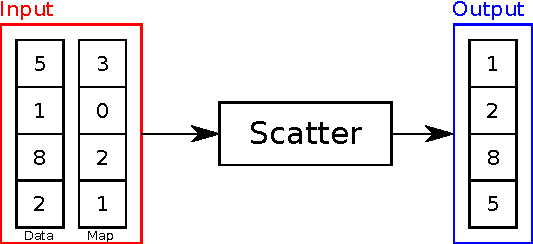
\includegraphics[height=0.6\textheight]{o_scatter}
\end{figure}

%https://thrust.github.io/doc/group__prefixsums.html
\begin{lstlisting}
thrust::scatter(data.begin(),data.end(),map.begin(),output.begin());
\end{lstlisting}
\end{frame}


\begin{frame}[fragile]
	\frametitle{Scatter}
	Sequential implementation on the CPU:
\begin{lstlisting}
void scatter(vector<T> data, vector<T> map, vector<T>& output)
{
	for(int i = 0; i < input.size(); ++i)
	{
		output[map[i]] = input[i];
	}
}
\end{lstlisting}
\end{frame}



\begin{frame}[fragile]
\frametitle{Scatter}
	\begin{itemize}
	\item Copy the input elements to the location given by a map
	\item<2-> Often used after a scan to \textit{compact} data
	\item<2-> \textbf{Example}: Convert the sparse matrix of rigid body collisions to a compact list
	\item<3-> Implementation:

\begin{lstlisting}
output[map[i]] = input[i];
\end{lstlisting}
	\item<3-> \href{https://thrust.github.io/doc/group__scattering.html}{Thrust API}
\end{itemize} 	
\end{frame}

\begin{frame}[fragile]
\frametitle{Gather}
\begin{figure}
	\centering
	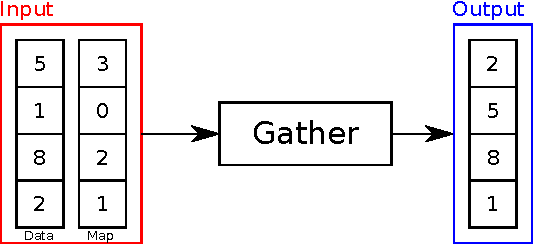
\includegraphics[height=0.6\textheight]{o_gather}
\end{figure}

%https://thrust.github.io/doc/group__prefixsums.html
\begin{lstlisting}
// output[i] = data[map[i]]
thrust::gather(data.begin(),data.end(),map.begin(),output.begin());
\end{lstlisting}
\end{frame}

\begin{frame}[fragile]
	\frametitle{Gather}
	Sequential implementation on the CPU:
\begin{lstlisting}
void gather(vector<T> data, vector<T> map, vector<T>& output)
{
	for(int i = 0; i < input.size(); ++i)
	{
		output[i] = input[map[i]];
	}
}
\end{lstlisting}
\end{frame}

\begin{frame}[fragile]
\frametitle{Gather}
\begin{itemize}
	\item The output element is the input indexed through a map
	\item<2-> Inverse operation of \textit{scatter}
	\item<3-> Implementation:


\begin{lstlisting}
output[i] = input[map[i]];
\end{lstlisting}
		\item<3-> \href{https://thrust.github.io/doc/group__gathering.html}{Thrust API}
\end{itemize} 
\end{frame}


\begin{frame}[fragile]
\frametitle{Compact}
\begin{figure}
	\centering
	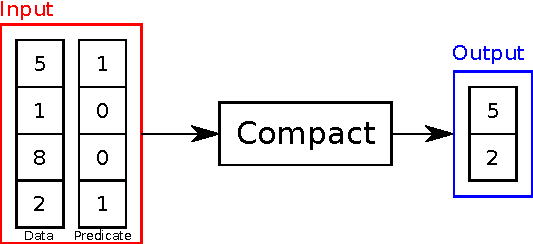
\includegraphics[height=0.6\textheight]{o_compact}
\end{figure}
\begin{lstlisting}
// Copy if the predicate is true
thrust::copy_if(data.begin(),data.end(),Predicate(),output.begin());
\end{lstlisting}
\end{frame}


\begin{frame}[fragile]
	\frametitle{Compact}
	Sequential implementation on the CPU:
\begin{lstlisting}
void copy_if(vector<T> data, OP predicate, vector<T>& output)
{
	for(int i = 0; i < input.size(); ++i)
	{
		if(predicate(data[i]))
		{
			output.push_back(data[i]);
		}
	}
}
\end{lstlisting}
\end{frame}

\begin{frame}[fragile]
\frametitle{Compact}
\begin{itemize}
	\item A predicate defines if the input element is copied to the output
	\item<2-> The order is retained
	\item<2-> The output array is sequential (no holes)
	\item<2-> \href{https://thrust.github.io/doc/group__stream__compaction.html}{Thrust API}
\end{itemize}
\onslide<3->
Implementation:
\begin{enumerate}
	\item Scan over the predicate
	\item Scatter elements to scanned offsets
\begin{lstlisting}
thrust::exclusive_scan(pred.begin(),pred.end(),map.begin());
thrust::scatter_if(data.begin(), data.end(), map.begin(), pred.begin(), out.begin());
\end{lstlisting}
\item [$\rightarrow$] Can be implemented in a single pass
\end{enumerate}
\end{frame}

\begin{frame}[fragile]
\frametitle{Thrust Compact Variants}

\begin{itemize}
\begin{lstlisting}
thrust::copy_if(first, last, result, pred);		
\end{lstlisting}
	\item Copy all elements in the range [first, last) to result for which the predicate evaluates to true
\begin{lstlisting}
thrust::copy_if(first, last, stencil, result, pred);		
\end{lstlisting}
\item Same as above except that the predicate is evaluated on the stencil
\end{itemize}
\end{frame}


\begin{frame}[fragile]
\frametitle{Sort}
\begin{figure}
	\centering
	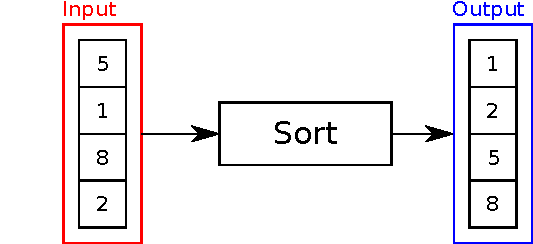
\includegraphics[height=0.6\textheight]{o_sort}
\end{figure}

%https://thrust.github.io/doc/group__prefixsums.html
\begin{lstlisting}
// In-place ascending sort
thrust::sort(data.begin(),data.end());
\end{lstlisting}
\end{frame}

\frame
{
	\frametitle{Sort}
	\begin{itemize}
		\item Sorting is very complex on the GPU
		\item Lots of communication between threads is required
		\item Communication in both directions (in contrast to Scan)
	\end{itemize}
\onslide<2->
2 different algorithms are present in this lecture:
\begin{itemize}
	\item<2-> Bitonic Sort for \textit{local} datasets (in warp, in block)
	\item<2-> Radix Sort for \textit{global} datasets
\end{itemize}
}

\frame
{
	\begin{mdframed}[frametitle={Bitonic Sequence}]
		A \textbf{Bitonic Sequence} is a sequence of numbers which is first increasing then after a point decreasing.
		\\ \\
		A \textbf{Bitonic Point} is a point in a bitonic sequence before which elements are increasing and after which elements are decreasing. A Bitonic point doesn’t exist if the array is only decreasing or only increasing.
	\end{mdframed}
}


\frame
{
		\frametitle{Bitonic Sequence}
		Is this sequence bitonic?
		\begin{itemize}
			\item<1-2>[] $[0, 1, 2, 1, 0]$ \onslide<2>{Yes}
			\item<3-4>[] $[5,4,3,2,1]$ \onslide<4>{Yes}
			\item<5-6>[] $[1, 1, 3, 2, 4]$ \onslide<6>{No}
			\item<7-8>[] $[0, 0,0, 100, 0, 0]$ \onslide<8>{Yes}
			\item<9-10>[] $[0, 5,5,4,5, 2, 1]$ \onslide<10>{No}
			\item<11-12>[] $[0]$ \onslide<12>{Yes}
			\item<13-14>[] $[8, 3]$ \onslide<14>{Yes}
		\end{itemize}
}

\frame
{
	\frametitle{Bitonic Sort}
\begin{itemize}
	\item The input consist of N bitonic sequences of size 2
	\item In each stage, neighboring sequences of the previous stage are merged
	\item After $\log_2(N)$ stages, a single increasing bitonic sequence remains

	\item[$\rightarrow$] Also called: \textit{Bitonic Merge Sort}
	\item[$\rightarrow$] Merging implemented with swap operations
\end{itemize}
}



\frame
{	
	\frametitle{Bitonic Sort}
	\begin{figure}
		\centering
		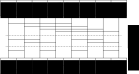
\includegraphics[height=0.8\textheight]{bitonic}
	\end{figure}
}


\frame
{
	\frametitle{Bitonic Sort (Stage 0)}
	\begin{figure}
		\centering
		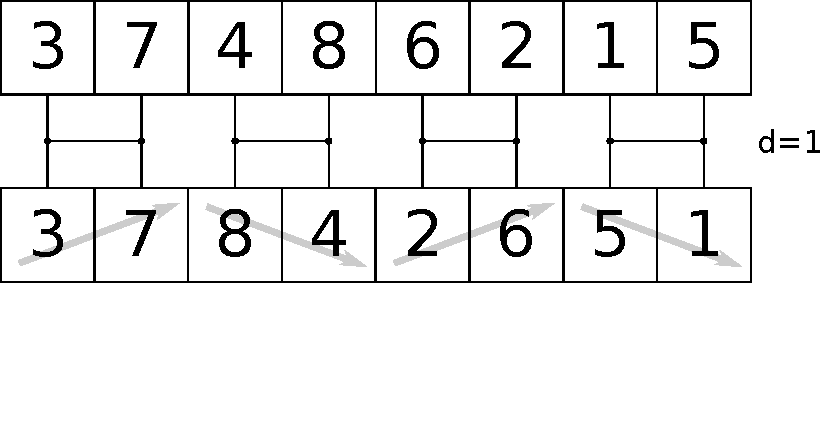
\includegraphics[height=0.6\textheight]{bitonic0}
	\end{figure}
}

\frame
{
	\frametitle{Bitonic Sort (Stage 1)}
	\begin{figure}
		\centering
		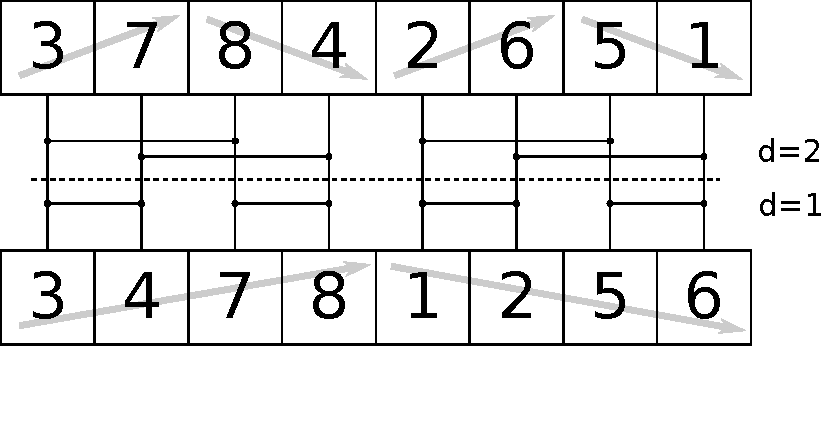
\includegraphics[height=0.6\textheight]{bitonic1}
	\end{figure}
}

\frame
{
	\frametitle{Bitonic Sort (Stage 2)}
	\begin{figure}
		\centering
		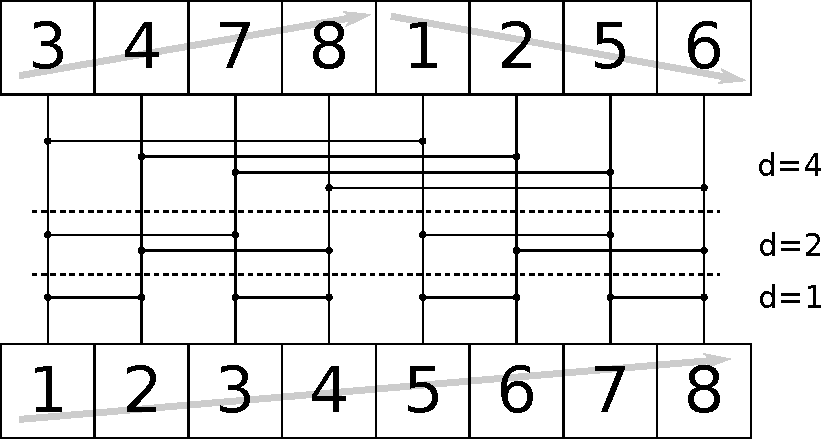
\includegraphics[height=0.6\textheight]{bitonic2}
	\end{figure}
}


\begin{frame}[fragile]
\frametitle{Bitonic Sort Implementation}
\begin{itemize}
	\item Swap elements of two threads
	\item The order is given by \texttt{direction}
\end{itemize}
\begin{lstlisting}
T shuffleSwapCompare(T x, int mask, int direction)
{
	auto y = Saiga::CUDA::shfl_xor(x,mask);
	return x < y == direction ? y : x;
}
\end{lstlisting}
\onslide<2->
\begin{itemize}
	\item Helper function to extract a single bit
\end{itemize}
\begin{lstlisting}
int bfe(int i , int k)
{
	return (i>>k) & 1;
}
\end{lstlisting}
\end{frame}

\begin{frame}[fragile]
\frametitle{Bitonic Sort Implementation}
\begin{lstlisting}
// l:= lane_id of this thread
T bitonicSortStage(T v, unsigned int stage,  unsigned int l)
{
	// Stage k requires (k+1) swaps
	for(auto i = 0; i <= stage; ++i)
	{
		// Half the distance in each iteration
		auto distance = 1 << (stage-i);
		
		// Some bit-magic to get the per-thread direction
		auto direction = bfe(l,stage-i) ^ bfe(l,stage+1);
		
		v = shuffleSwapCompare(v,distance,direction);
	}
	return v;
}
\end{lstlisting}
\end{frame}


\begin{frame}[fragile]
\frametitle{Bitonic Sort Implementation}
\begin{lstlisting}
T bitonicWarpSort(T v, unsigned int l)
{
	// Sorting 32 elements requries log(32)=5 stages
	for(int stage = 0; stage < 5 ; ++stage)
	{
		v = bitonicSortStage(v,stage,l);
	}
	return v;
}
\end{lstlisting}
\href{https://github.com/darglein/saiga/blob/master/samples/cuda/bitonicSort/main.cu}{Full Source + Example @ GitHub}
\end{frame}

\frame
{
	\frametitle{Bitonic Sort Implementation}
\begin{itemize}
	\item Implementation on blocks:
	\begin{enumerate}
		\item The first 5 stages in a warp 
		\item<2-> Copy all values to shared memory
		\item<2-> Sort in shared memory (syncThreads after each swap)
	\end{enumerate}
\onslide<3->
\item Global Bitonic sort
\begin{enumerate}
	\item A global sync is required after every swap
	\item<4->[$\rightarrow$] Very inefficient
\end{enumerate}
\end{itemize}
}

\frame
{
	\frametitle{Radix Sort}
	\begin{itemize}
		\item Sort elements into $k$ buckets
		\item Count the number of elements in each bucket and reorder the array
		\item Iterate $log_k(M)$ times, where $M$ is the number of possible values
		\item Also know as Counting Sort, Bucket Sort
		\item<2-> In the following example:
\begin{itemize}
	\item<2-> 2 buckets (one for each bit)
	\item<2-> 8 possible values $\rightarrow$ 3 stages
\end{itemize}
	\end{itemize}
}

\frame
{
	\frametitle{Radix Sort}
	\begin{figure}
		\centering
		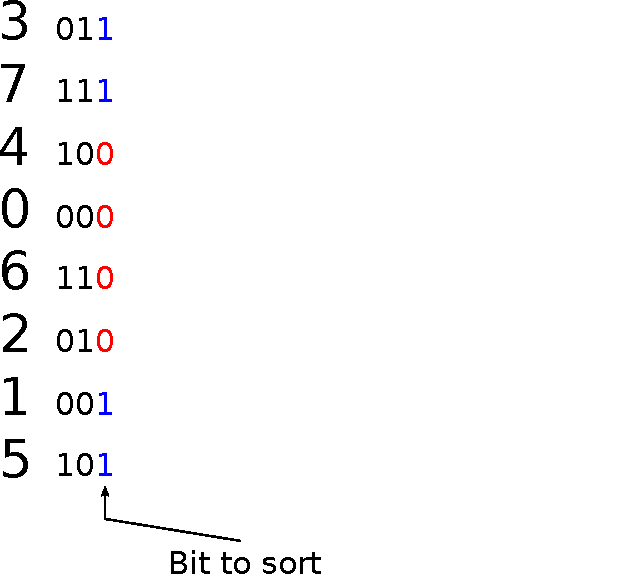
\includegraphics[height=0.7\textheight]{radix0}
	\end{figure}
}

\frame
{
	\frametitle{Radix Sort}
	\begin{figure}
		\centering
		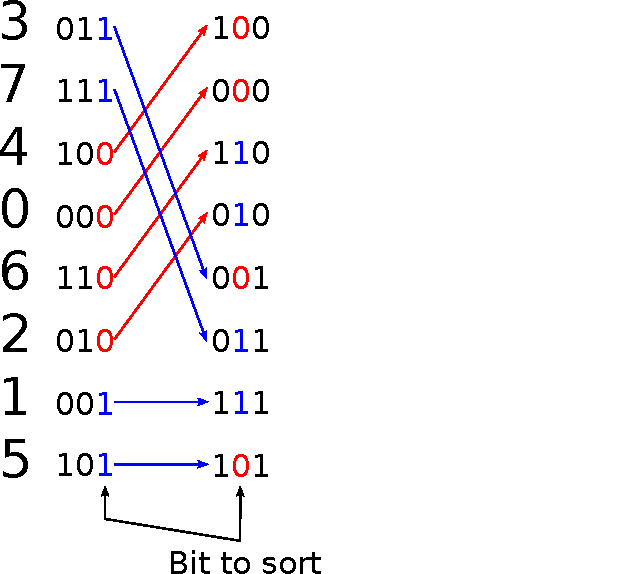
\includegraphics[height=0.7\textheight]{radix1}
	\end{figure}
}

\frame
{
	\frametitle{Radix Sort}
	\begin{figure}
		\centering
		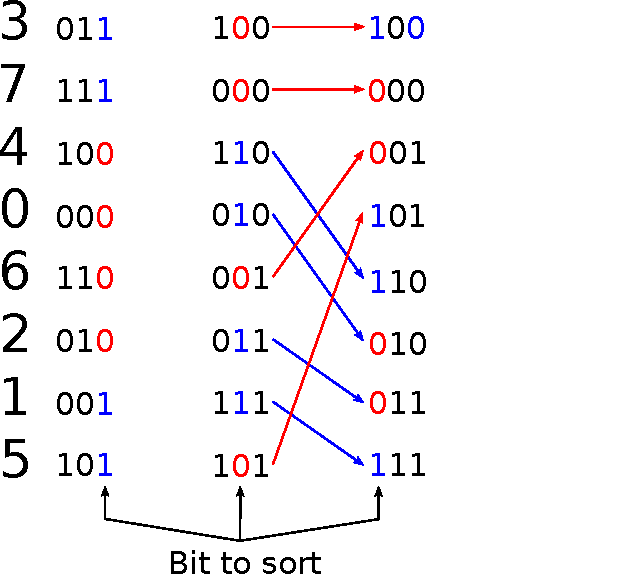
\includegraphics[height=0.7\textheight]{radix2}
	\end{figure}
}

\frame
{
	\frametitle{Radix Sort}
	\begin{figure}
		\centering
		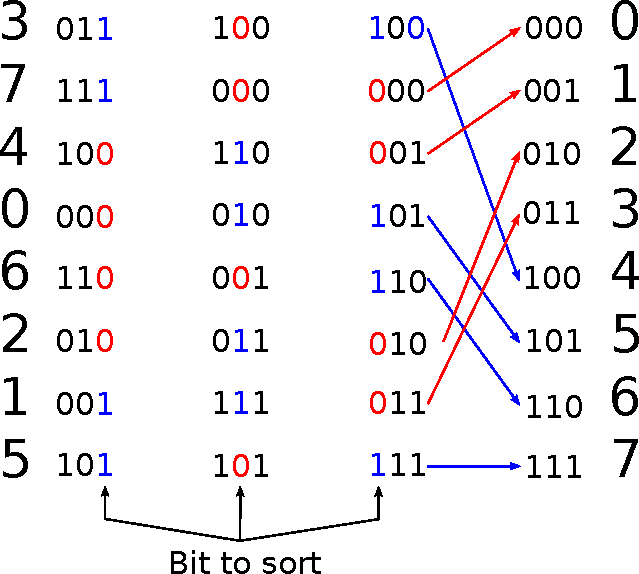
\includegraphics[height=0.7\textheight]{radix3}
	\end{figure}
}

\frame
{
	\frametitle{Radix Sort (single step)}
	\begin{figure}
		\centering
		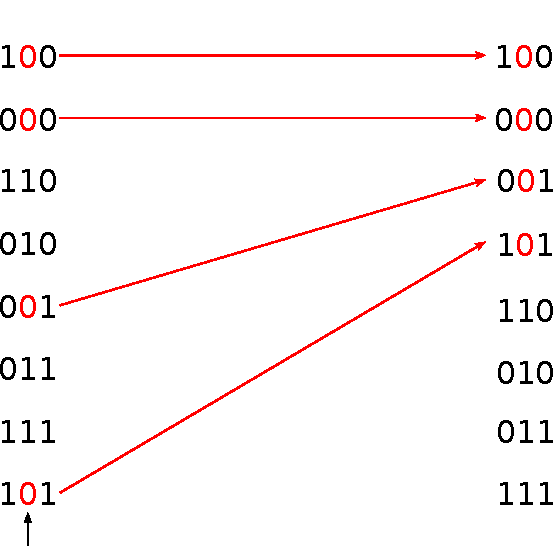
\includegraphics[height=0.7\textheight]{radix4}
	\end{figure}
}

\frame
{
	\frametitle{Radix Sort (single step)}
	\begin{figure}
		\centering
		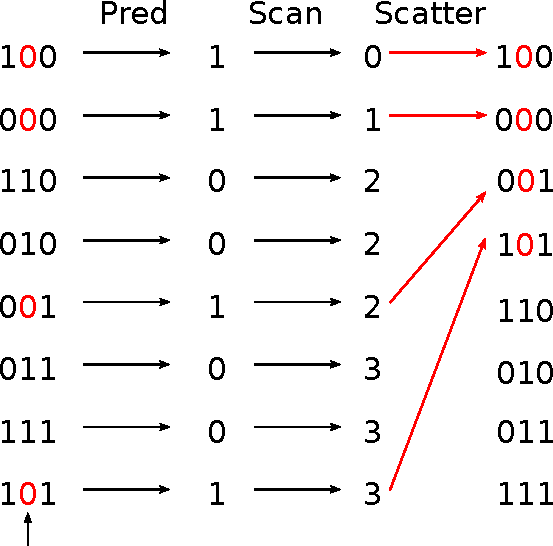
\includegraphics[height=0.7\textheight]{radix5}
	\end{figure}
}

\frame
{
	\frametitle{Radix Sort (single step)}
	\begin{figure}
		\centering
		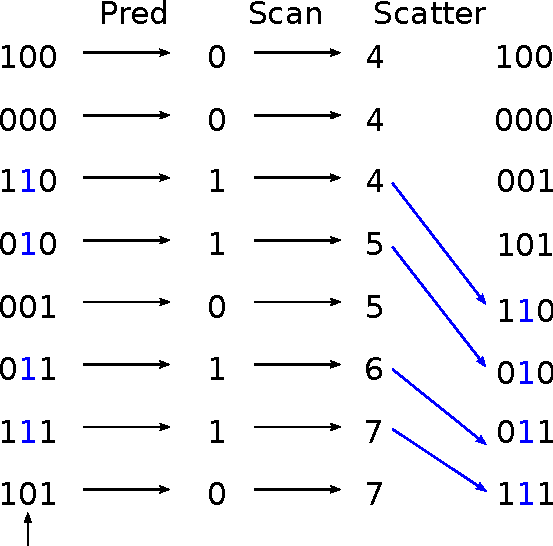
\includegraphics[height=0.7\textheight]{radix6}
	\end{figure}
}

\begin{frame}[fragile]
\begin{itemize}
	\item Implementation with thrust functions
\end{itemize}
\begin{lstlisting}
static void radixSort(ArrayView<int> data)
{
	int N = data.size();
	
	thrust::device_vector<int> temp(N);

	// Sort from least to most significant bit
	for(int i = 0; i < 32; ++i)
		radixSortHelper(data,temp,i);
}

\end{lstlisting}
\end{frame}


\begin{frame}[fragile]
\begin{itemize}
	\item Operator to extract a single bit $k$ from the integer
\end{itemize}
\begin{lstlisting}
template<bool one>
struct GetBitOp
{
	int k;
	GetBitOp(int k) : k(k){}
	HD inline int operator()(int a){
		return ((a >> k) & 1) == one;
	}
};
\end{lstlisting}
\end{frame}

\begin{frame}[fragile]

\begin{lstlisting}
static void radixSortHelper(...)
{
	// Copy the numbers with 0 as the current bit to the beginning of t
	auto it = thrust::copy_if(
		d.begin(),d.end(),t.begin(),GetBitOp<false>(bit));
	
	// Place the numbers with 1 as the current bit after the 0s
	thrust::copy_if(d.begin(),d.end(),it,GetBitOp<true>(bit));
	
	// The scan-scatter radix sort does not work inplace!
	thrust::copy(t.begin(),t.end(),d.begin());
}
\end{lstlisting}

\href{https://github.com/darglein/saiga/blob/master/samples/cuda/radixSort/main.cu}{Full Source + Example @ GitHub}
\end{frame}




\begin{frame}[fragile]
	\frametitle{Radix Sort - Conclusion}
	\begin{itemize}
		\item Radix sorts works well on parallel architectures
		\item We can implement a global radix sort with compact operations!
		\item Real radix sort implementations are more optimized:
		\begin{itemize}
			\item sorting by multiple bits in each step
			\item combining the 0- and 1-compaction
			\item[$\rightarrow$] Lots of papers have been written about GPU sorts. 
			\href{https://ieeexplore.ieee.org/abstract/document/5161005}{Link}
		\end{itemize}
	\item Don't implement a global sort by yourself!
	\item[$\rightarrow$] Use thrust in your program:
\begin{lstlisting}
thrust::sort(data.begin(),data.end());
\end{lstlisting}
	\end{itemize}
\end{frame}

 	
\begin{frame}[fragile]
\frametitle{Thrust Sort Variants}

\begin{itemize}
\begin{lstlisting}
thrust::is_sorted(first, last);		
\end{lstlisting}
	\item is\_sorted returns true if the range [first, last) is sorted in ascending order, and false otherwise.
\begin{lstlisting}
thrust::sort(first, last, [comp]);		
\end{lstlisting}
\item Sorts the elements in [first, last) into ascending order
\begin{lstlisting}
thrust::stable_sort(first, last, [comp]);		
\end{lstlisting}
\item Same as sort but relative order stays unchanged
\begin{lstlisting}
thrust::sort_by_key(keys_first, keys_last, values_first, [comp]);
\end{lstlisting}
\item Sorts the keys and(!) values. Only the values are use for comparison.
\end{itemize}
\url{https://thrust.github.io/doc/group__sorting.html}
\end{frame}

\frame{
	\frametitle{Literature}
	%
	\begin{itemize}
		\item \href{https://docs.nvidia.com/cuda/}{Cuda Toolkit Documentation}
		\item \href{https://thrust.github.io/doc/group__algorithms.html}{Thrust Algorithms}
		\item \href{https://github.com/darglein/saiga}{Saiga}
		\item \href{https://research.nvidia.com/sites/default/files/pubs/2016-03_Single-pass-Parallel-Prefix/nvr-2016-002.pdf}{Scan (Paper)}
		\item \href{http://on-demand.gputechconf.com/gtc/2013/presentations/S3174-Kepler-Shuffle-Tips-Tricks.pdf}{Shuffle Tips and Tricks}
		\item \href{https://nvlabs.github.io/cub/}{CUB Documentation}
	\item		\href{https://ieeexplore.ieee.org/abstract/document/5161005}{GPU Sort}
	\end{itemize}
	
}





\end{document}



